\section{Требования к среде выполнения}\label{sec:deploy}

\begin{frame}{Требования к среде выполнения}

    \begin {itemize}
    \item \textbf{Простота}
    \begin{itemize}
        \item \textit{Локальная разработка}
        \item \textit{Администрирование}
        \item \textit{Решение проблем}
    \end{itemize}

    \item \textbf{Изолированность}
    \item \textbf{Переносимость}
    \item \textbf{Управляемость}
    \begin{itemize}
        \item \textit{Переменные окружения}
        \item \textit{Управление версиями}
        \item \textit{Логирование и мониторинг}
    \end{itemize}

    \item \textbf{Масштабируемость}
    \begin{itemize}
        \item \textit{Вертикальное масштабирование}
        \item \textit{Горизонтальное масштабирование}
    \end{itemize}

    \end{itemize}

\end{frame}

\begin{frame}{ Эволюция деплоя приложений}

    \begin{figure}
        \centering
        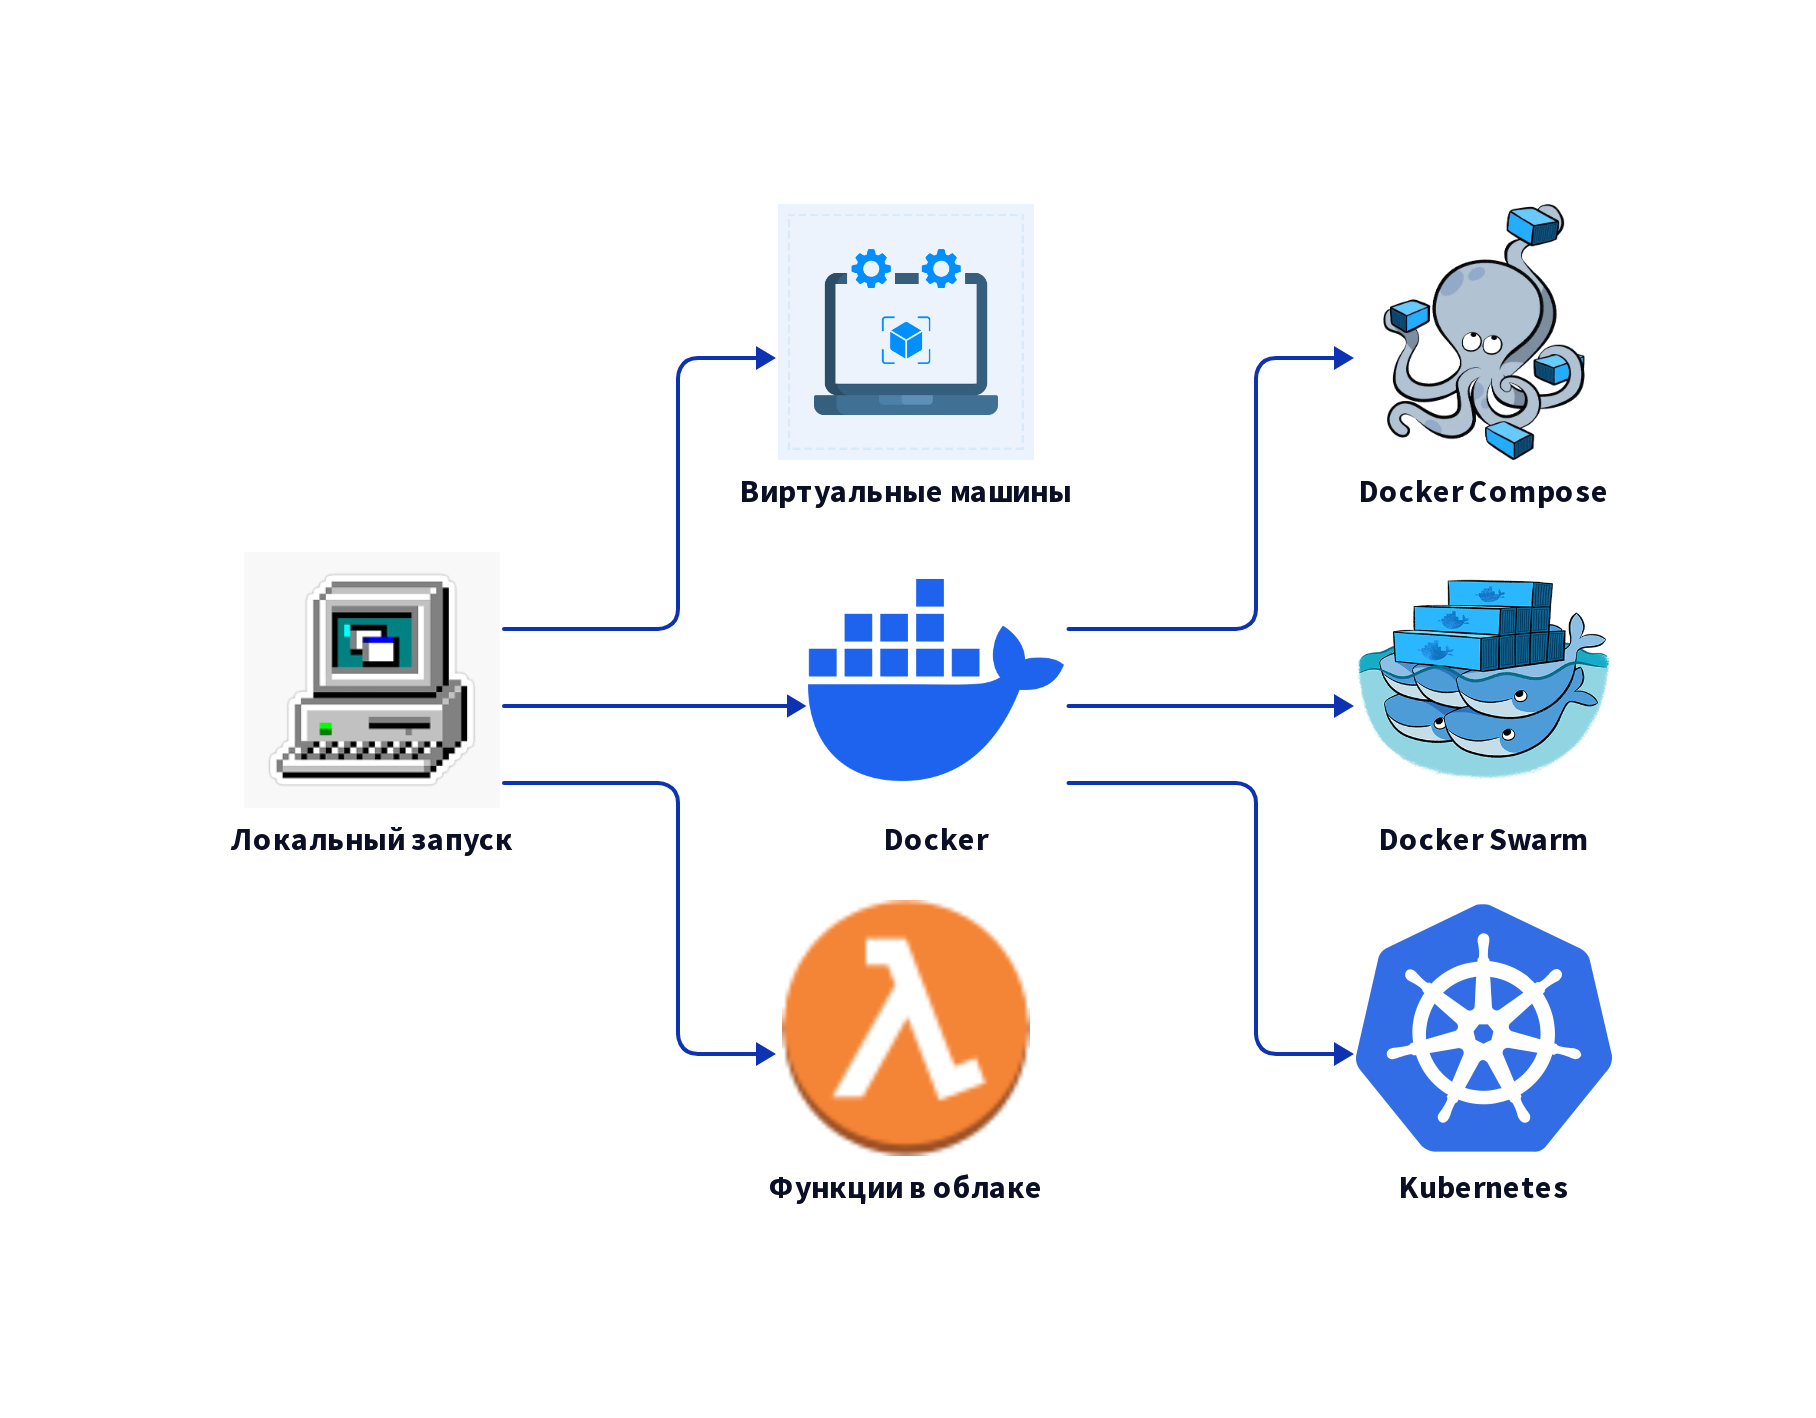
\includegraphics[width=\paperheight]{images/docker.png}
        \label{fig:evolution}
    \end{figure}

\end{frame}



\section{Docker Compose vs Docker Swarm}\label{sec:comparison}
\begin{frame}{Docker Compose vs Docker Swarm}
    \begin{table}[]
        \begin{tabular}{lcc}
            \multicolumn{1}{c}{\textbf{Качество}}  & \textbf{Docker Compose} & \textbf{Docker Swarm} \\
            Сложность                              & легко                   & чуть сложнее          \\
            Поддержка зависимостей между сервисами & \yes                    & \no                   \\
            Поддержка репликации                   & \no                     & \yes                  \\
            Поддержка кластеризации                & \no                     & \yes                  \\
            Прозрачное обновления сервисов         & \no                     & \yes                  \\
            Балансировщик нагрузки                 & \no                     & \yes                  \\
            Дополнительные требования к приложению & \no                     & \yes
        \end{tabular}
    \end{table}

    Требования Docker Swarm к приложению и деплою:
    \begin{itemize}
        \item Обработка недоступности других сервисов (БД, Redis, ...)
        \item Наличие healthcheck у сервисов
        \item Обработка сигналов \texttt{SIGTERM}/\texttt{SIGKILL}
    \end{itemize}

\end{frame}

